\documentclass{beamer}
\usetheme{CambridgeUS}
%\usepackage[brazil]{babel}
\usepackage[utf8]{inputenc}
\usepackage{graphicx}
\title{Arboviroses: Elimine o Mosquito!}
\author{Baseado na cartilha da Fiocruz}
\date{}

\begin{document}

\frame{\titlepage}

\begin{frame}{O que são arboviroses?}
    \begin{itemize}
        \item Doenças causadas por vírus transmitidos por insetos (vetores).
        \item No Brasil, as mais comuns são:
        \begin{itemize}
            \item Dengue
            \item Zika
            \item Chikungunya
        \end{itemize}
        \item Todas são transmitidas pelo mosquito Aedes aegypti.
    \end{itemize}
\end{frame}

\begin{frame}{Quem é o Aedes aegypti?}
    \begin{itemize}
        \item Mosquito com listras brancas no corpo e pernas.
        \item Coloca ovos em água parada.
        \item Pica principalmente durante o dia.
    \end{itemize}
    \begin{center}
        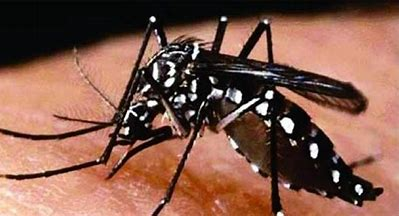
\includegraphics[width=0.5\textwidth]{aedes.jpg} % Substitua com a imagem adequada
    \end{center}
\end{frame}

\begin{frame}{Diferenças entre as doenças}
    \begin{tabular}{|p{2.5cm}|p{3.5cm}|p{3.5cm}|}
        \hline
        \textbf{Doença} & \textbf{Sintomas principais} & \textbf{Consequências} \\
        \hline
        Dengue & Febre alta, dor atrás dos olhos, dor muscular intensa & Hemorragias, Dengue grave (pode ser fatal) \\
        \hline
        Zika & Manchas vermelhas, coceira, febre leve & Microcefalia em bebês (caso infecte gestantes), problemas neurológicos \\
        \hline
        Chikungunya & Febre alta, dores articulares fortes & Dor crônica nas articulações, pode durar meses \\
        \hline
    \end{tabular}
\end{frame}

\begin{frame}{Como eliminar o mosquito}
    \begin{itemize}
        \item Tampar caixas d’água
        \item Jogar fora água acumulada em pneus e garrafas
        \item Limpar calhas e ralos
        \item Usar telas em janelas
    \end{itemize}
    \pause
    \centering
    \textbf{Pequenas ações salvam vidas!}
\end{frame}

\begin{frame}{Atividade em grupo: Criação de Cartazes}
    \textbf{Tema: "Nesse campeonato, o eliminado é o mosquito!"}
    \vspace{0.3cm}
    \begin{itemize}
        \item Materiais:
        \begin{itemize}
            \item Cartolina colorida.
            \item Tinta, canetões, lápis de cor.
        \end{itemize}
        \item Organização:
        \begin{itemize}
            \item Formem grupos de até 5 alunos.
            \item Criem um cartaz educativo sobre como combater o mosquito.
            \item Usem a criatividade: desenhos, colagens, slogans!
        \end{itemize}
    \end{itemize}
    \vfill
    \textit{Os melhores cartazes serão expostos na escola!}
\end{frame}

\begin{frame}{Resumo da aula}
    \begin{itemize}
        \item Arboviroses são um problema sério de saúde pública.
        \item O combate ao mosquito começa em casa.
        \item Conhecimento e ação fazem a diferença.
    \end{itemize}
    \pause
    \centering
    \textbf{\Large Vamos agir juntos!}
\end{frame}

\end{document}

